
\chapter{Methodology}
\section{High Level Design}
\subsection{Block Diagram}

The MetaGPT framework follows a sophisticated multi-tier architecture that supports distributed agent interactions, intelligent communication protocols, and RAG-enhanced knowledge processing. The system is organized into clearly defined layers that collaborate to transform user requirements into validated code artifacts.

\begin{figure}[H]
    \centering
    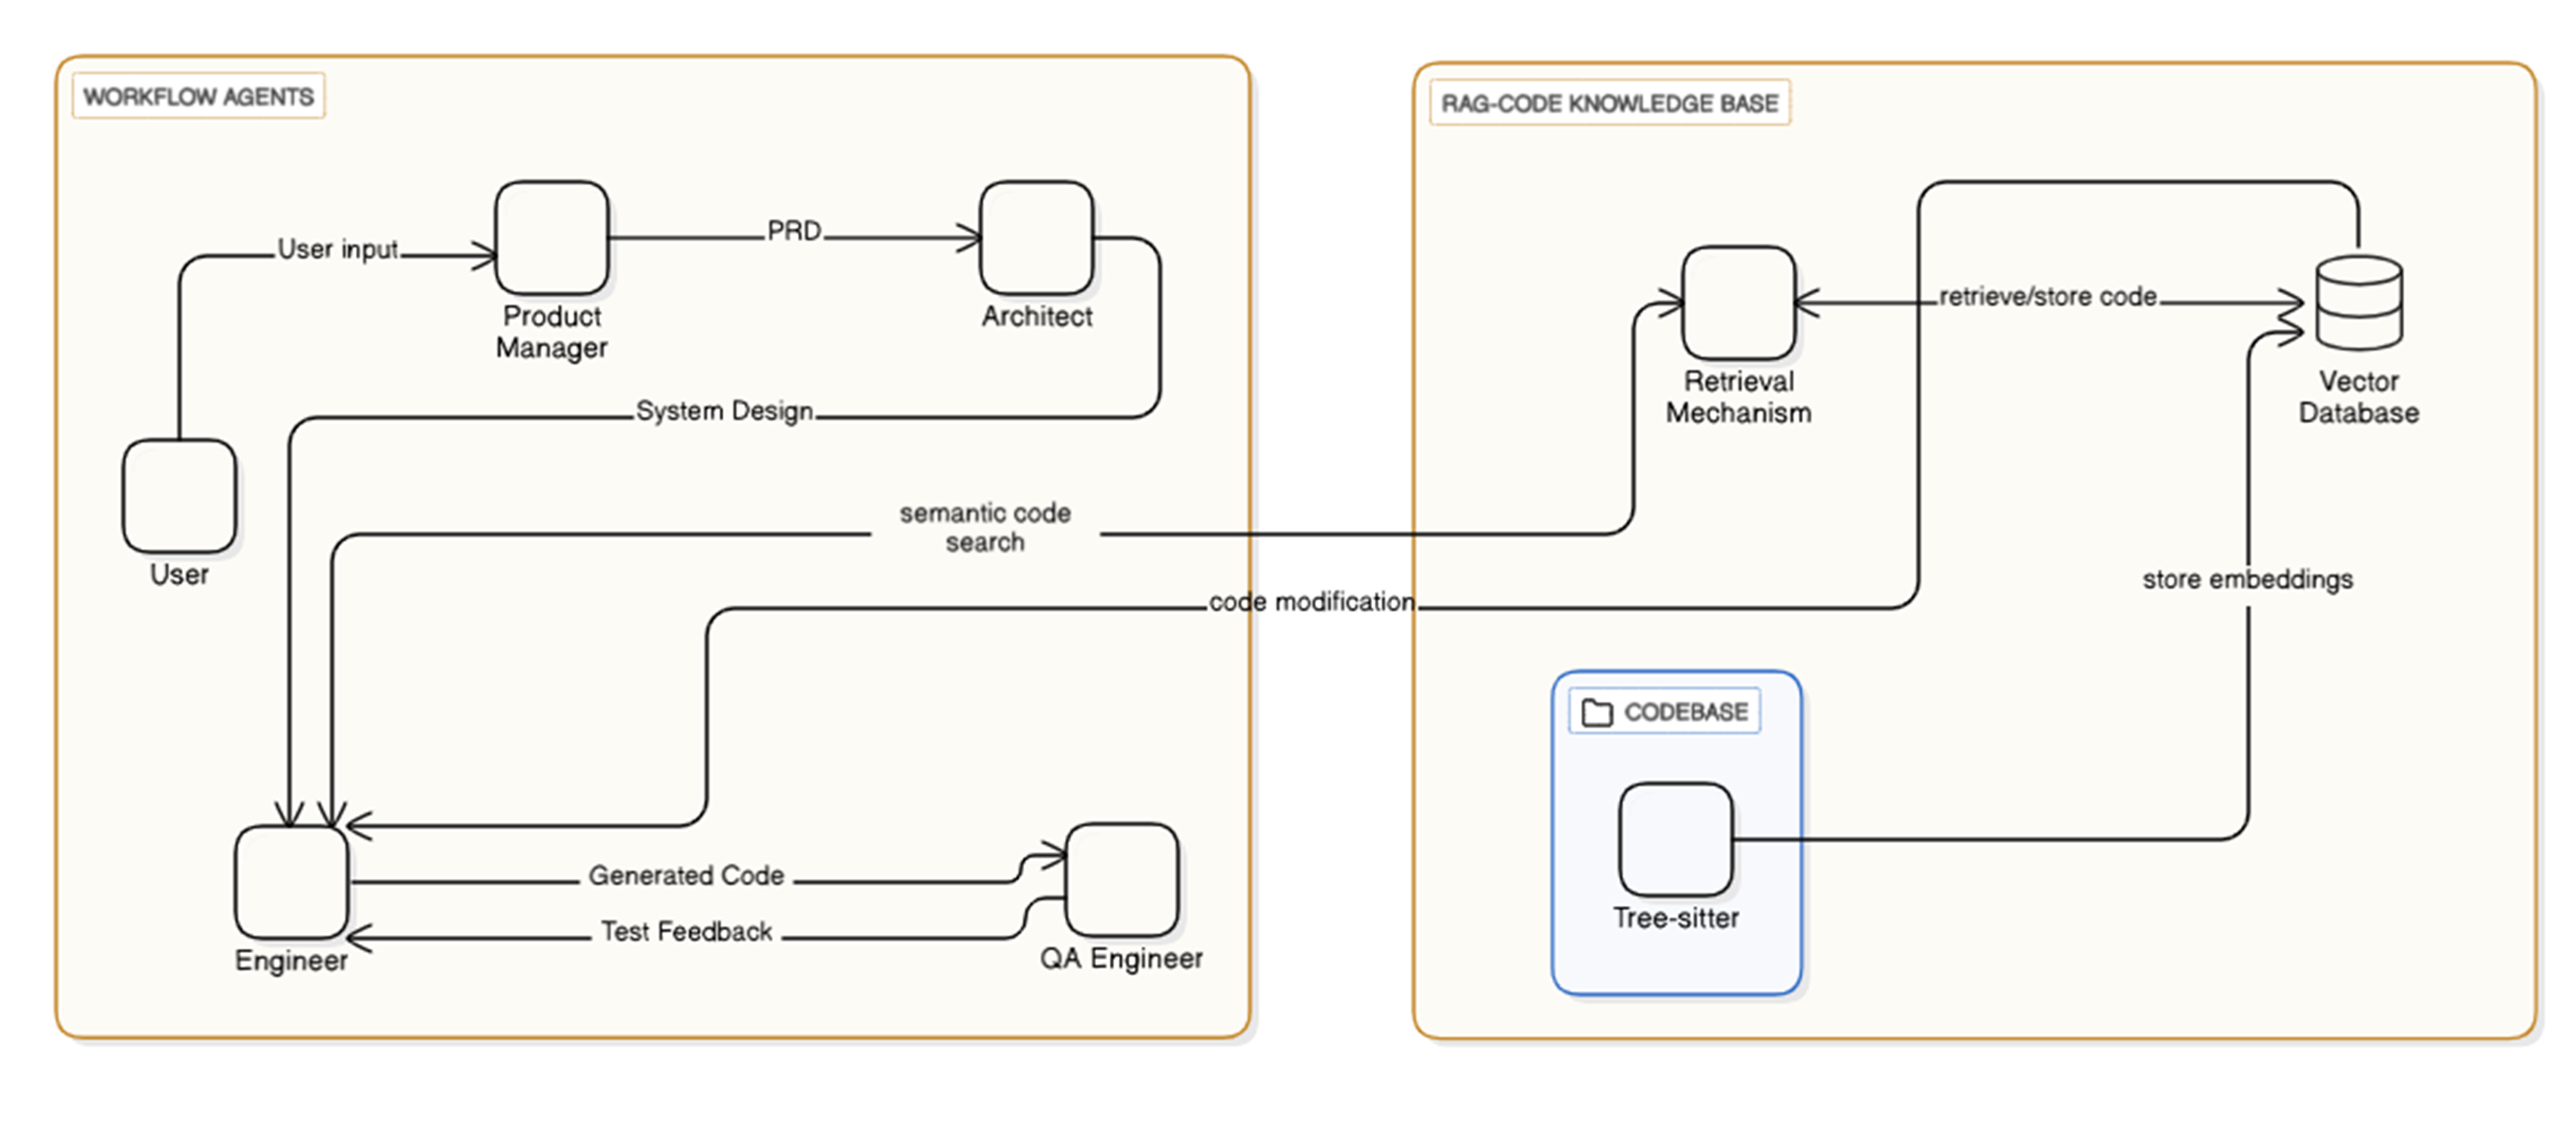
\includegraphics[width=0.9\textwidth]{images/arch.png}
    \caption{High-Level MetaGPT System Architecture}
    \label{fig:architecture}
\end{figure}

The architecture diagram in Figure~\ref{fig:architecture} illustrates the following key components:

\begin{itemize}
    \item \textbf{Frontend Layer:} React-based user interface providing agent management, workflow visualization, and real-time collaboration monitoring.
    \item \textbf{API Gateway:} FastAPI backend serving as the central orchestration point for all agent interactions and workflow management.
    \item \textbf{Agent Framework:} LangGraph-based state graph providing deterministic agent orchestration, with LangChain used as the LLM abstraction layer for calling Google Gemini.
    \item \textbf{Specialized Agents:} Manager, Architect, Engineer, and QA agents with distinct roles and responsibilities.
    \item \textbf{RAG System:} Vector database integration with semantic search capabilities for context-aware code generation and knowledge retrieval.
    \item \textbf{AI Integration:} Gemini API integration providing state-of-the-art language model capabilities for agent reasoning and code generation.
    \item \textbf{Communication Layer:} Shared-state passing via a pipeline service, where each agent reads typed outputs from the previous agent and writes its own output into the same state object.
\end{itemize}


\subsection{Use Case Diagram}

The Use Case diagram illustrates the interactions between the primary actors (User and Multi-Agent System) and the MetaGPT framework, showing the complete software development lifecycle from user input to final code delivery.

\begin{figure}[H]
    \centering
    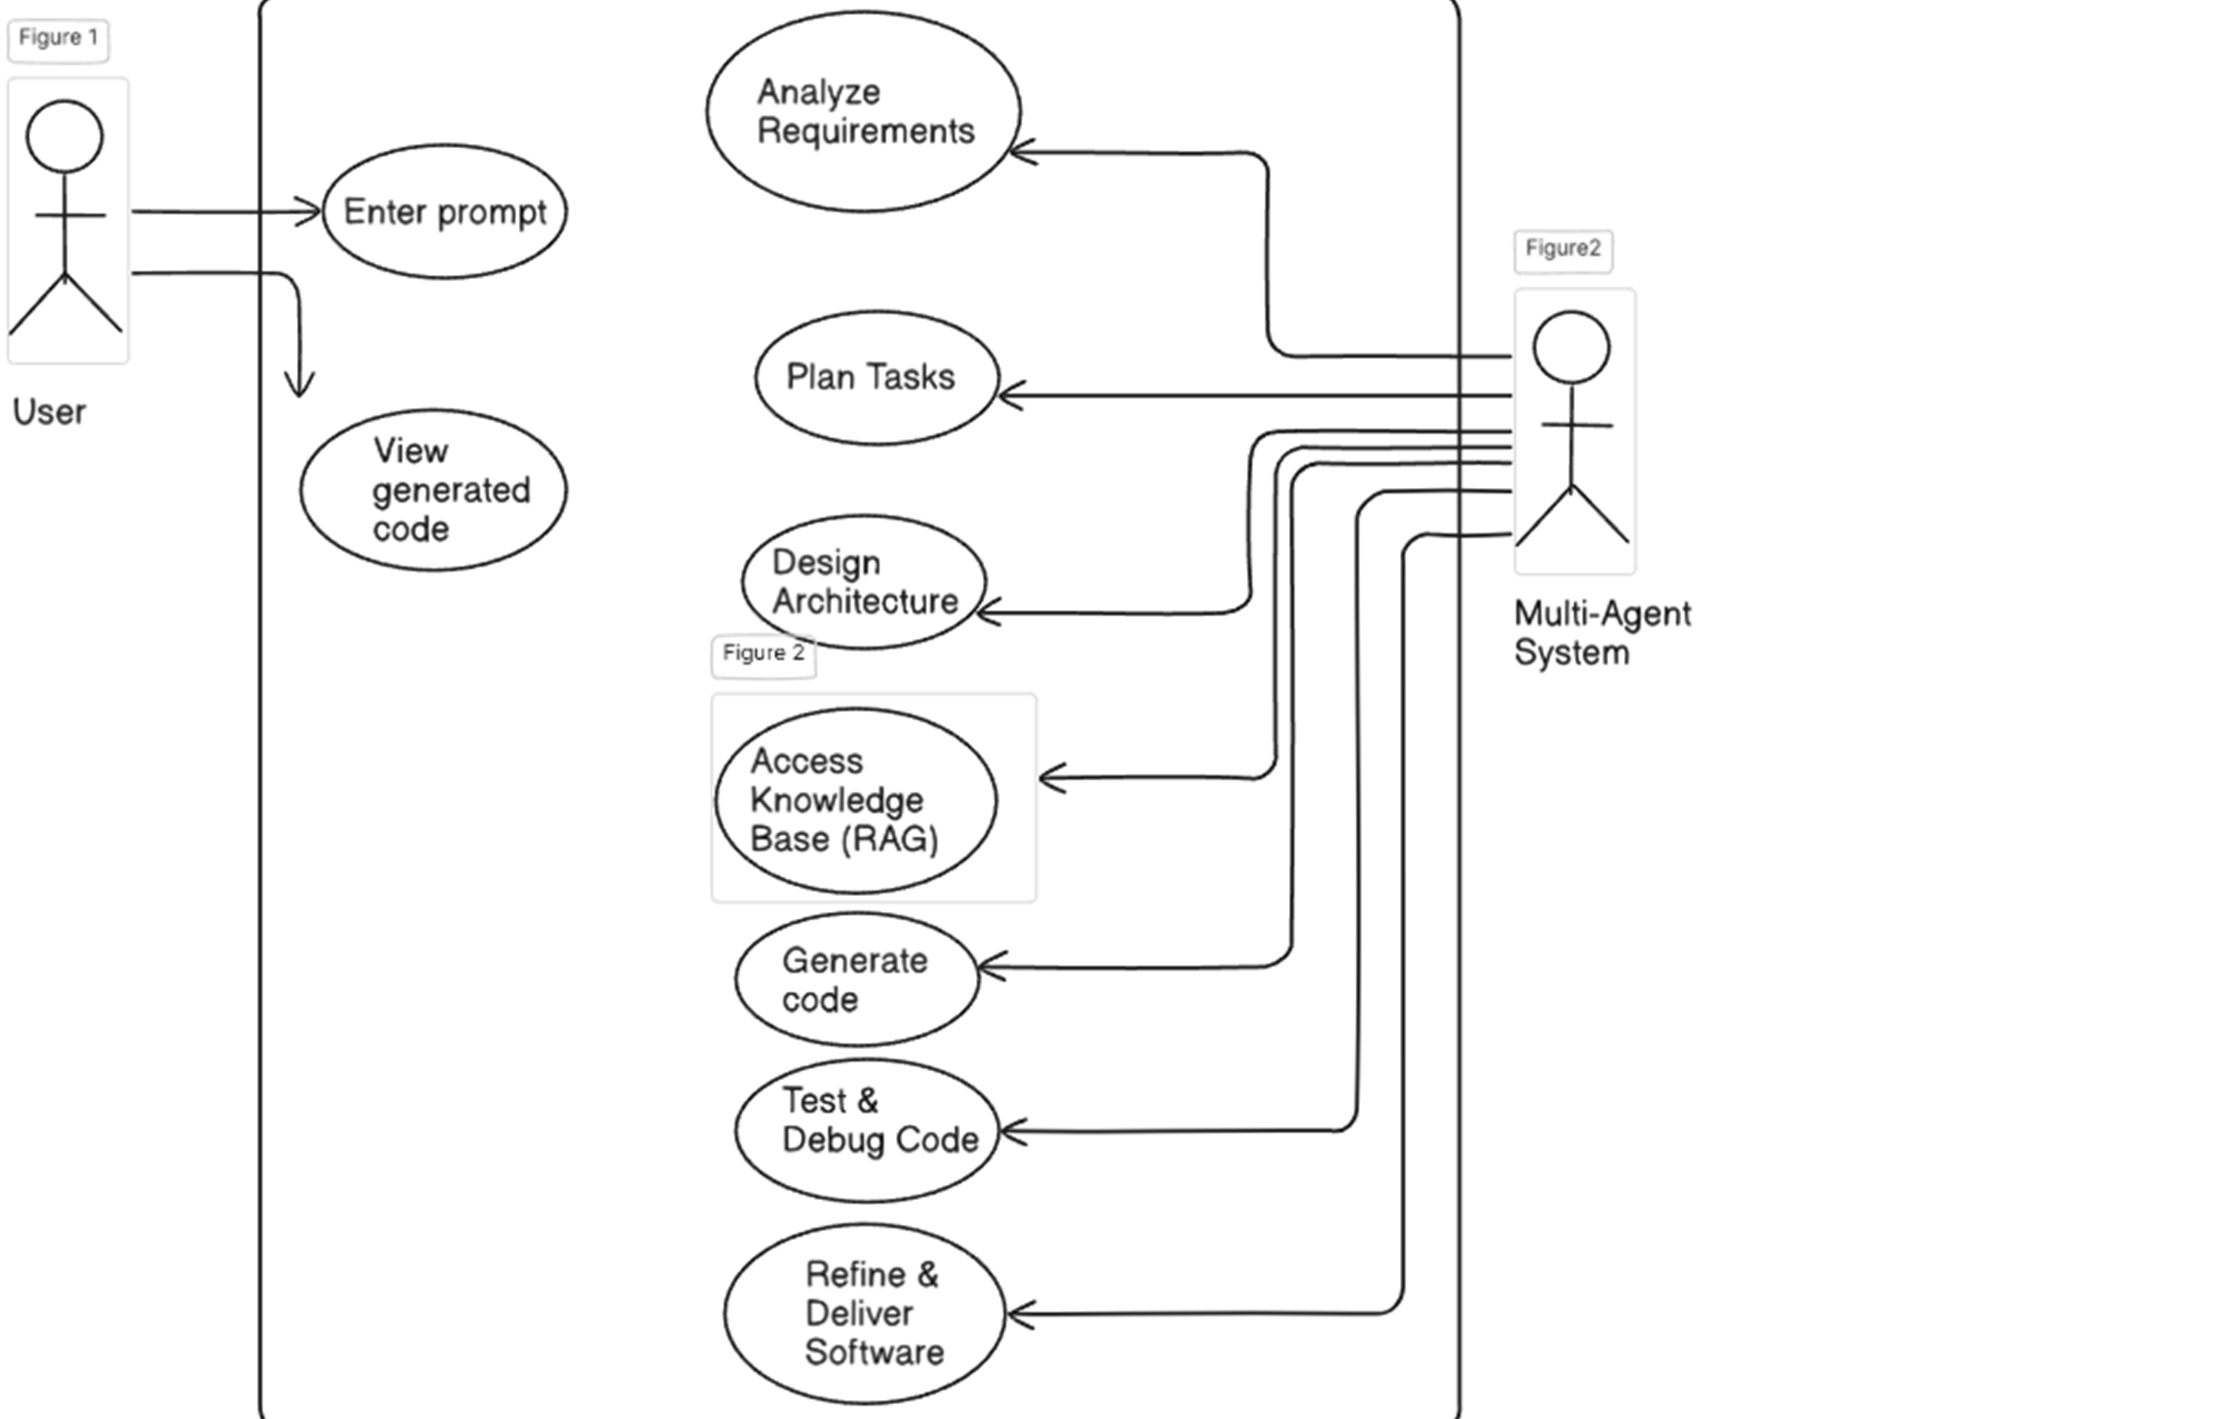
\includegraphics[width=0.8\textwidth]{images/use_case_diagram.png}
    \caption{MetaGPT System Use Case Diagram}
    \label{fig:use_case}
\end{figure}


\section{Detailed Design}
\subsection{Module 1: Backend API Layer}

The first major module is the \textbf{Backend API Layer}, implemented using FastAPI under the \texttt{backend/\allowbreak{}app} package. Its primary responsibility is to expose a stable HTTP interface for all core operations, including project management, pipeline execution, file access, chat-based iteration, and retrieval-augmented generation.

The entry point \texttt{main.py} constructs the FastAPI application, configures middleware, and includes the top-level router defined in \texttt{api/\allowbreak{}router.py}. The router aggregates versioned endpoints under the \texttt{/\allowbreak{}api/\allowbreak{}v1} prefix, delegating to individual endpoint modules such as:
\begin{itemize}
    \item \texttt{api/\allowbreak{}endpoints/\allowbreak{}projects.py} for creating, listing, and retrieving projects.
    \item \texttt{api/\allowbreak{}endpoints/\allowbreak{}pipeline.py} for running the agentic pipeline in batch or streaming mode.
    \item \texttt{api/\allowbreak{}endpoints/\allowbreak{}files.py} for browsing the project file tree and fetching or updating file contents.
    \item \texttt{api/\allowbreak{}endpoints/\allowbreak{}chat.py} for handling iterative chat interactions tied to a project.
    \item \texttt{api/\allowbreak{}endpoints/\allowbreak{}rag.py} and \texttt{api/\allowbreak{}endpoints/\allowbreak{}sandbox.py} for RAG and sandbox-related operations.
\end{itemize}

Each endpoint module validates incoming requests using Pydantic schemas from the \texttt{schemas} package, calls into dedicated service functions, and returns structured responses. Authentication and authorization concerns are centralized in \texttt{auth.py} and integrated into endpoint dependencies where required.

In addition to the core project/pipeline/files/chat endpoints, MetaGPT implements sandbox management endpoints in \texttt{api/\allowbreak{}endpoints/\allowbreak{}sandbox.py} to support live previews of generated projects. The sandbox workflow is intentionally non-blocking: the \texttt{/\allowbreak{}{project\_\allowbreak{}id}/create} endpoint returns \textbf{202 Accepted} immediately and triggers sandbox creation as a background task, while clients poll \texttt{/\allowbreak{}{project\_\allowbreak{}id}/status} until the sandbox becomes \texttt{ready} and a \texttt{preview\_\allowbreak{}url} is available. This design prevents request timeouts during dependency installation and dev-server startup.

\subsection{Module 2: Agent Orchestration and Graph}

The second module is the \textbf{Agent Orchestration and Graph Module}, which coordinates the sequence of Manager, Architect, Engineer, and QA agents using LangGraph. The overall pipeline state is defined in \texttt{graph/\allowbreak{}state.py}, where a central data structure captures the prompt, intermediate artifacts, agent outputs, and final project representation.

The orchestration logic in \texttt{graph/\allowbreak{}orchestrator.py} builds a directed graph whose nodes correspond to individual agents and whose edges represent valid transitions. For example, the Manager node takes a raw user prompt and produces a structured requirement specification, which becomes input to the Architect node. The Architect node generates a high-level system design and file plan, which is passed to the Engineer node to create concrete source files. Finally, the QA node inspects the generated artifacts, produces test cases, and records quality-related feedback.

The orchestrator integrates with LangChain’s LLM abstractions to call Google Gemini via helper functions defined in the \texttt{llm} module. It also records intermediate outputs so that the frontend can display an execution timeline and visualizations of agent reasoning. Error handling, retries, and logging are centralized here, making the pipeline robust and easier to debug or extend with additional agents in the future.

\subsection{Module 3: Storage and Project Management}

The third module is the \textbf{Storage and Project Management Module}, which persists all artifacts produced by the pipeline and exposes higher-level operations for managing projects. This module is implemented primarily in the \texttt{storage} and \texttt{models} packages.

Domain models such as \texttt{models/\allowbreak{}project.py} and \texttt{models/\allowbreak{}user.py} describe core entities, while storage backends in \texttt{storage/\allowbreak{}project\_\allowbreak{}store.py} and \texttt{storage/\allowbreak{}file\_\allowbreak{}store.py} handle reading and writing data. Project state is persisted in \textbf{MongoDB} using the Beanie ODM (with Motor as the async driver), as implemented in \texttt{db.py}, \texttt{models/\allowbreak{}project.py}, and \texttt{storage/\allowbreak{}project\_\allowbreak{}store.py}. The project store is responsible for:
\begin{itemize}
    \item Creating a new project directory structure in a configurable \texttt{PROJECTS\_\allowbreak{}DIR} for generated code files.
    \item Recording metadata such as project identifiers, associated prompts, and timestamps in MongoDB.
    \item Listing existing projects and resolving paths for files within a given project.
\end{itemize}

The file store provides operations to:
\begin{itemize}
    \item Generate a tree representation of project files for the frontend file explorer.
    \item Read file contents for display in the code viewer.
    \item Apply updates to files when users edit code through the interface.
\end{itemize}

Together, these components decouple persistent storage concerns from the agent pipeline and API layer. This persistence layer stores project metadata, pipeline status, and agent outputs (including generated files), enabling recovery after server restarts and supporting long-running workflows. When ephemeral disk cache is missing, the pipeline service can restore project files from MongoDB back to disk so that file browsing and preview remain functional.

\subsection{Module 4: Frontend User Interface}

The fourth module is the \textbf{Frontend User Interface}, implemented with Next.js, TypeScript, and Tailwind CSS under the \texttt{frontend/\allowbreak{}src} directory. It provides an interactive, dark-themed workspace where users can manage projects and visualize the behavior of the agent pipeline.

The App Router structure in \texttt{src/\allowbreak{}app} defines key pages:
\begin{itemize}
    \item \texttt{page.tsx} as the landing page for entering prompts and viewing recent projects.
    \item \texttt{projects/\allowbreak{}page.tsx} for listing all projects retrieved from the backend.
    \item \texttt{project/\allowbreak{}[id]/\allowbreak{}page.tsx} as the main workspace for a specific project, showing files, agent outputs, and chat.
    \item \texttt{signin/\allowbreak{}page.tsx} and \texttt{signup/\allowbreak{}page.tsx} for authentication flows (if enabled).
\end{itemize}

Reusable components in \texttt{src/\allowbreak{}components} encapsulate major UI features:
\begin{itemize}
    \item \texttt{FileExplorer.tsx} renders the project tree and allows users to select files.
    \item \texttt{CodeViewer.tsx} displays syntax-highlighted source code and possibly supports editing.
    \item \texttt{AgentOutputs.tsx} shows structured reasoning and outputs from each agent in the pipeline.
    \item \texttt{ExecutionTimeline.tsx} visualizes the sequence and status of agent executions.
    \item \texttt{ChatPanel.tsx} enables iterative conversations tied to a particular project.
\end{itemize}

Client-side state is managed using stores defined in \texttt{src/\allowbreak{}lib/\allowbreak{}store.ts} and related files, while API communication is abstracted in \texttt{src/\allowbreak{}lib/\allowbreak{}api.ts}. Global styles and Tailwind configuration ensure a consistent look-and-feel across the application.

\subsection{Module 5: LLM, SOP, and Retrieval}

The fifth module is the \textbf{LLM, SOP, and Retrieval Module}, which encapsulates all logic related to configuring the underlying LLM, defining agent SOPs, and supporting retrieval-augmented generation (RAG). This module ties together the conceptual behavior of agents with concrete model calls and knowledge sources.

The \texttt{llm/\allowbreak{}gemini.py} file provides helper functions such as \texttt{get\_\allowbreak{}llm} and \texttt{get\_\allowbreak{}llm\_\allowbreak{}with\_\allowbreak{}structured\_\allowbreak{}output}, which create LangChain-compatible LLM instances backed by Google Gemini. Configuration values such as model name, temperature, maximum tokens, and API key are read from \texttt{config.py} and environment variables, ensuring that model behavior can be tuned without changing application code.

Agent behaviors are specified in \texttt{sop/\allowbreak{}definitions.py}, where each agent’s role, objectives, inputs, outputs, constraints, and quality checklist are documented. These SOPs are consumed by the agent implementations in the \texttt{agents} package, providing a clear contract between high-level design and concrete prompts issued to the LLM.

The RAG submodule in \texttt{rag} contains utilities for indexing and retrieving relevant documents. Files such as \texttt{rag/\allowbreak{}indexer.py}, \texttt{rag/\allowbreak{}vector\_\allowbreak{}store.py}, \texttt{rag/\allowbreak{}retriever.py}, and \texttt{rag/\allowbreak{}embeddings.py} manage the creation of vector embeddings, storage of vectors, and retrieval of context for augmenting LLM prompts. This enables MetaGPT to ground agent reasoning in existing project artifacts or external knowledge bases, improving accuracy and consistency for complex tasks.

\section{Data Flow Diagram}

Data Flow Diagrams (DFDs) illustrate the movement of data within the MetaGPT system and how information flows between different agents and components.

\subsection{Context Diagram (Level 0 DFD)}
The Level 0 DFD illustrates the high-level interaction between the User and the MetaGPT system, showing the complete workflow from user input to final code delivery.

\begin{figure}[H]
    \centering
    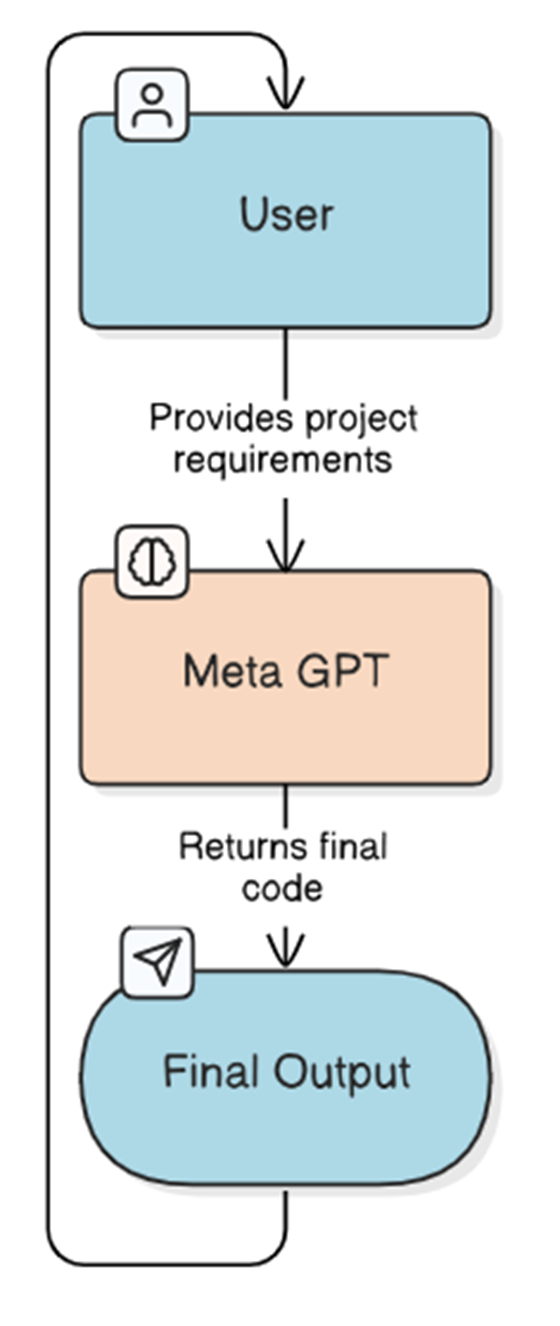
\includegraphics[width=0.3\textwidth]{images/dfd_level_0_final.png}
    \caption{DFD Level 0 - MetaGPT System}
    \label{fig:dfd_0}
\end{figure}

\subsection{Level 1 DFD}
The Level 1 DFD illustrates the internal workings of the MetaGPT system, showing how specialized agents collaborate to transform user requirements into validated code output through structured workflows and iterative feedback loops.

\begin{figure}[H]
    \centering
    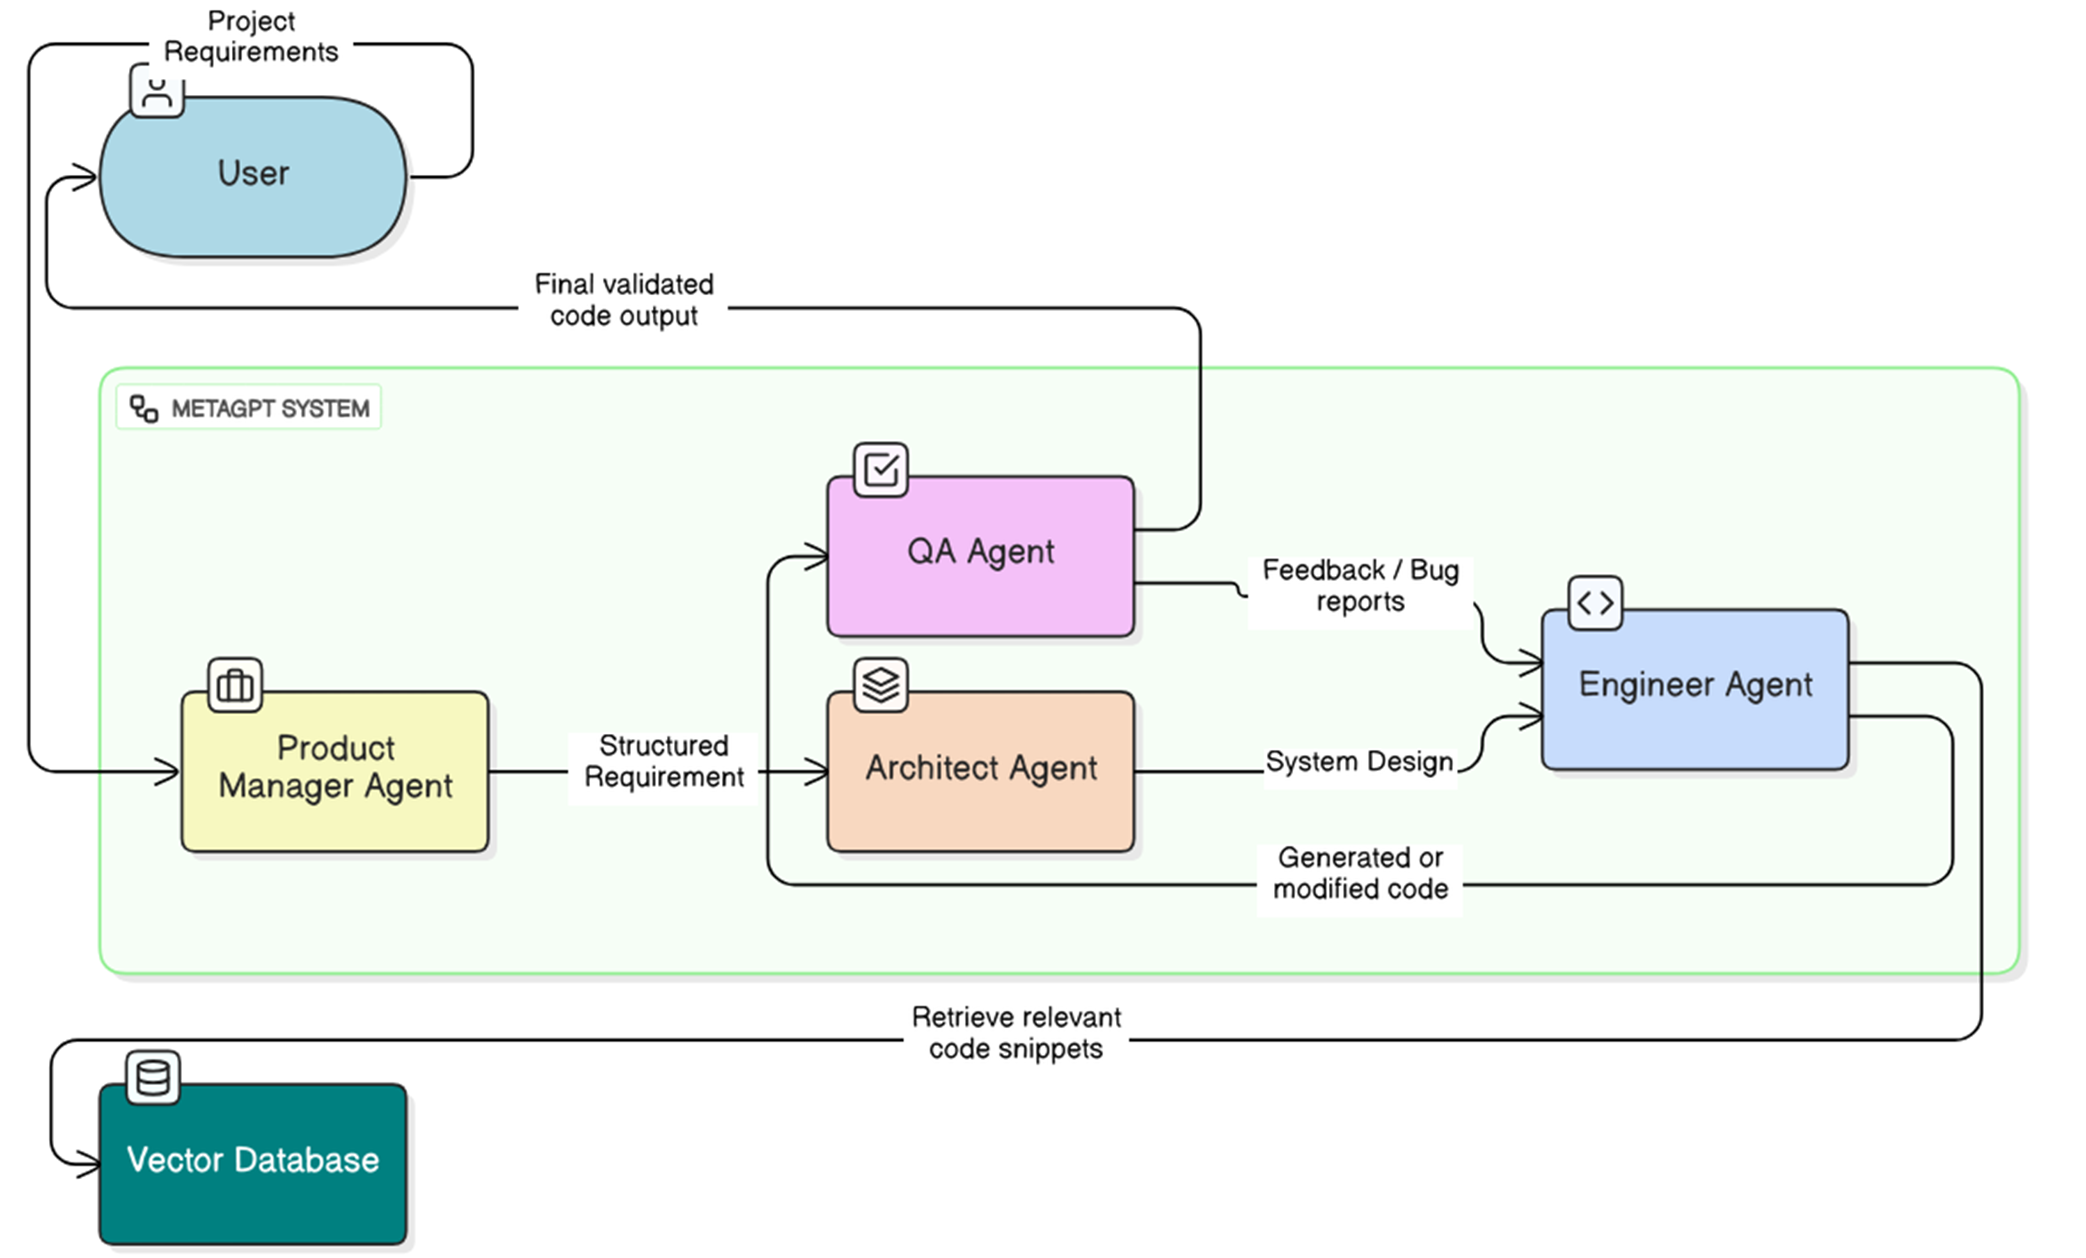
\includegraphics[width=1.0\textwidth]{images/dfd_level_1_final.png}
    \caption{DFD Level 1 - MetaGPT System Internal Workflow}
    \label{fig:dfd_1}
\end{figure}

\subsection{Level 2 DFD}

The Level 2 Data Flow Diagram provides a detailed decomposition of the MetaGPT system's internal agent collaboration process, showing the granular data flows and transformations that occur within each agent's specialized workflow.

\begin{figure}[H]
    \centering
    \makebox[\textwidth]{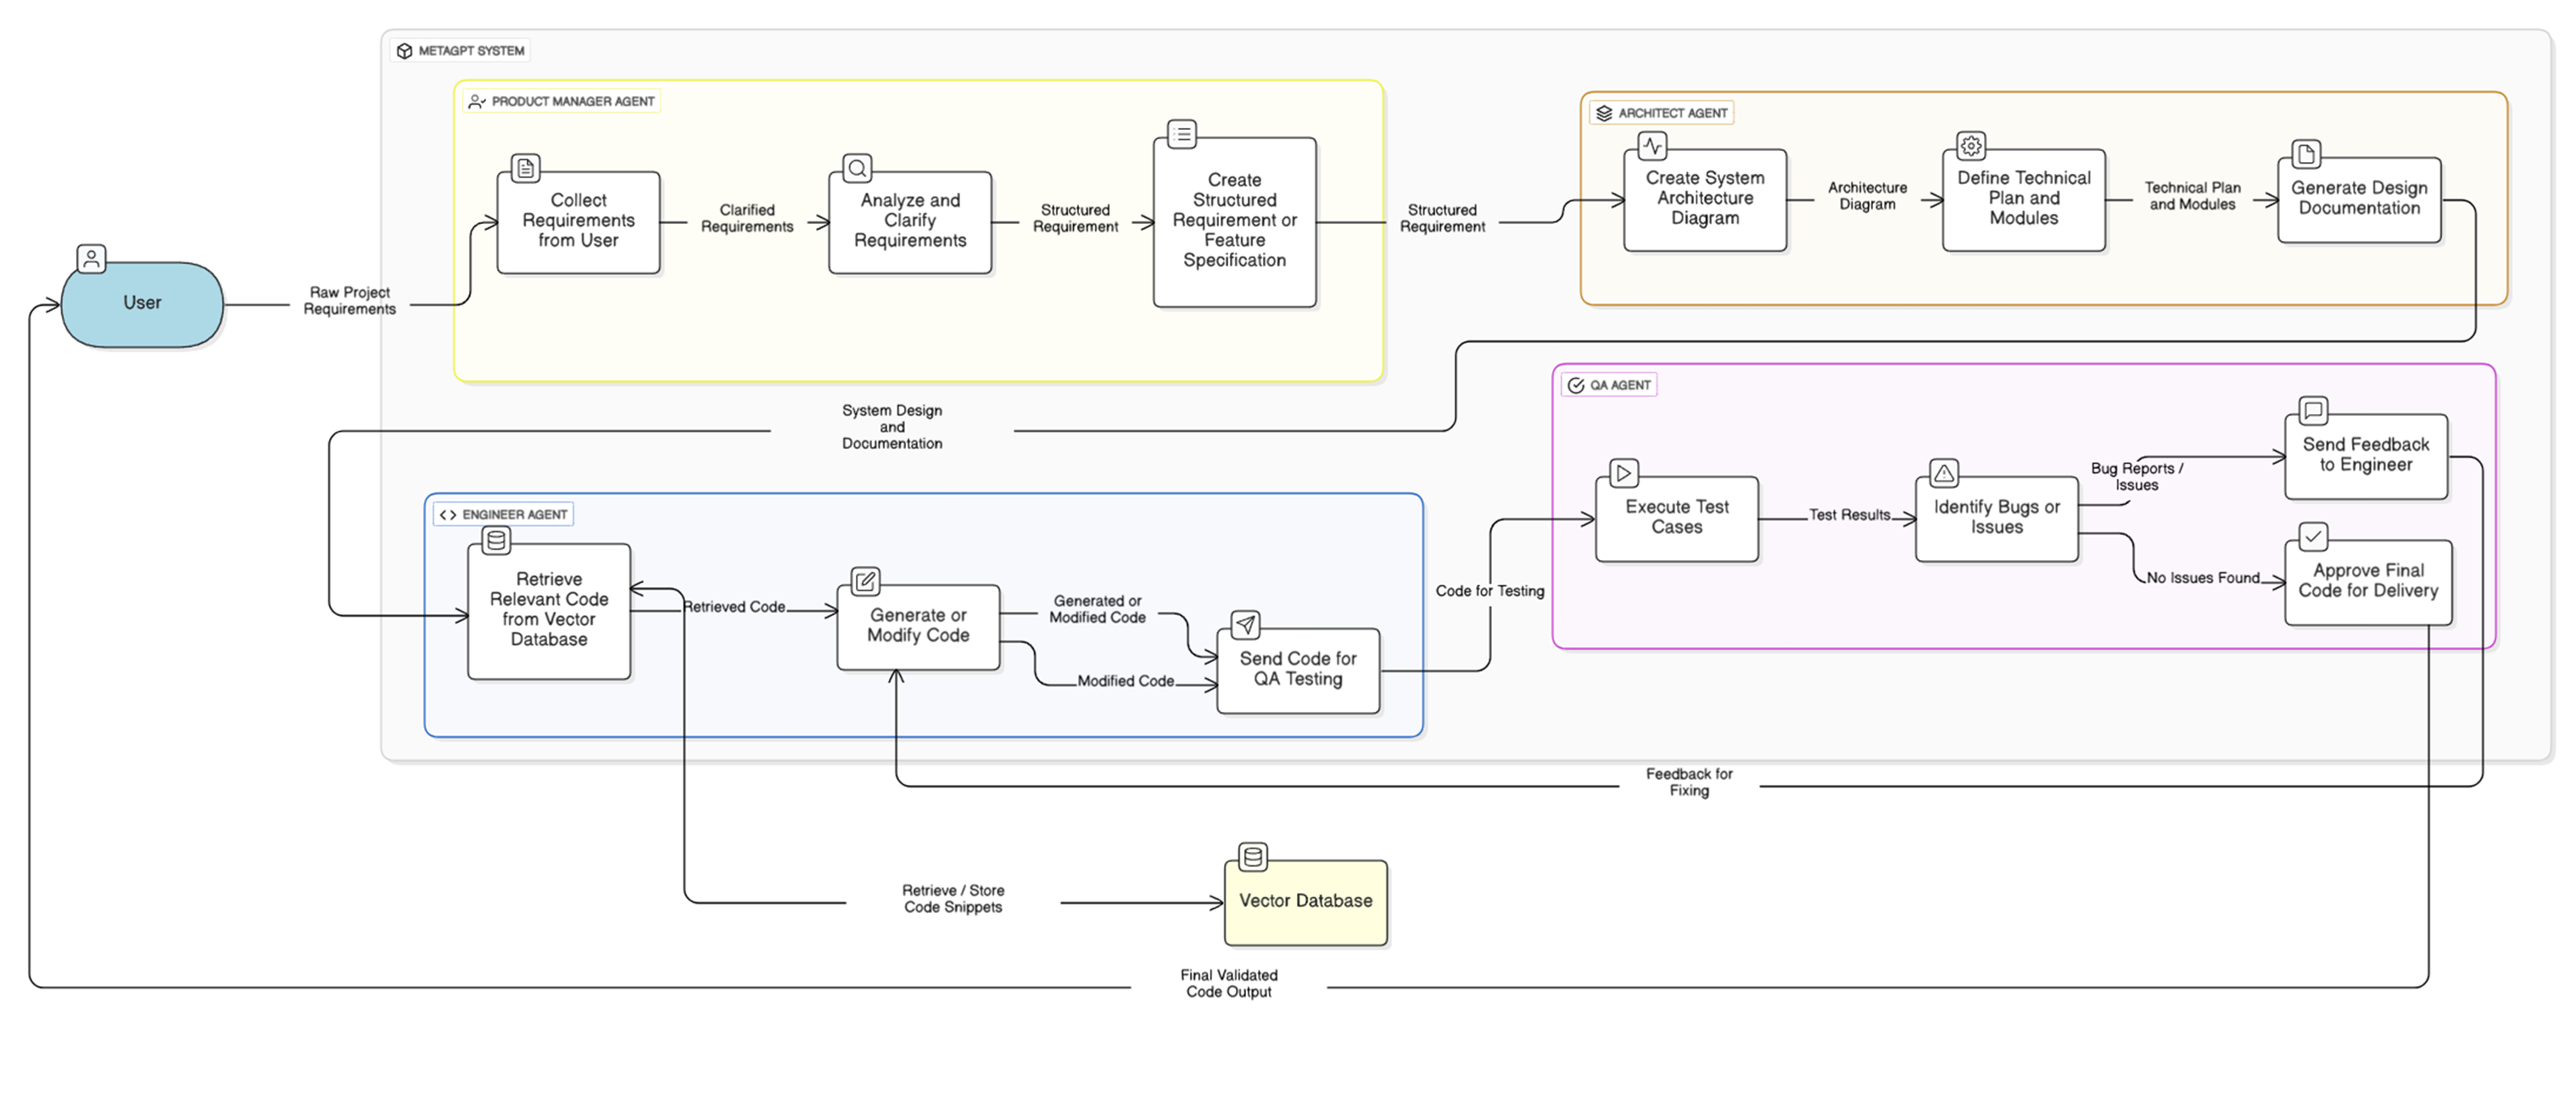
\includegraphics[width=\paperwidth]{images/dfd2.png}}
    \caption{DFD Level 2 — Detailed Agent Collaboration Process}
    \label{fig:dfd_2}
\end{figure}

\section{ER Diagram}

Lorem ipsum dolor sit amet, consectetur adipiscing elit. 
Sed do eiusmod tempor incididunt ut labore et dolore magna aliqua. 
Ut enim ad minim veniam, quis nostrud exercitation ullamco laboris nisi ut aliquip ex ea commodo consequat. 
Duis aute irure dolor in reprehenderit in voluptate velit esse cillum dolore eu fugiat nulla pariatur. 
Excepteur sint occaecat cupidatat non proident, sunt in culpa qui officia deserunt mollit anim id est laborum.

\section{UI Design}

The User Interface (UI) is designed to be clean, modern, and intuitive, prioritizing the agent management and workflow visualization experience. The following screenshots illustrate the key screens of the application.

\begin{figure}[H]
    \centering
    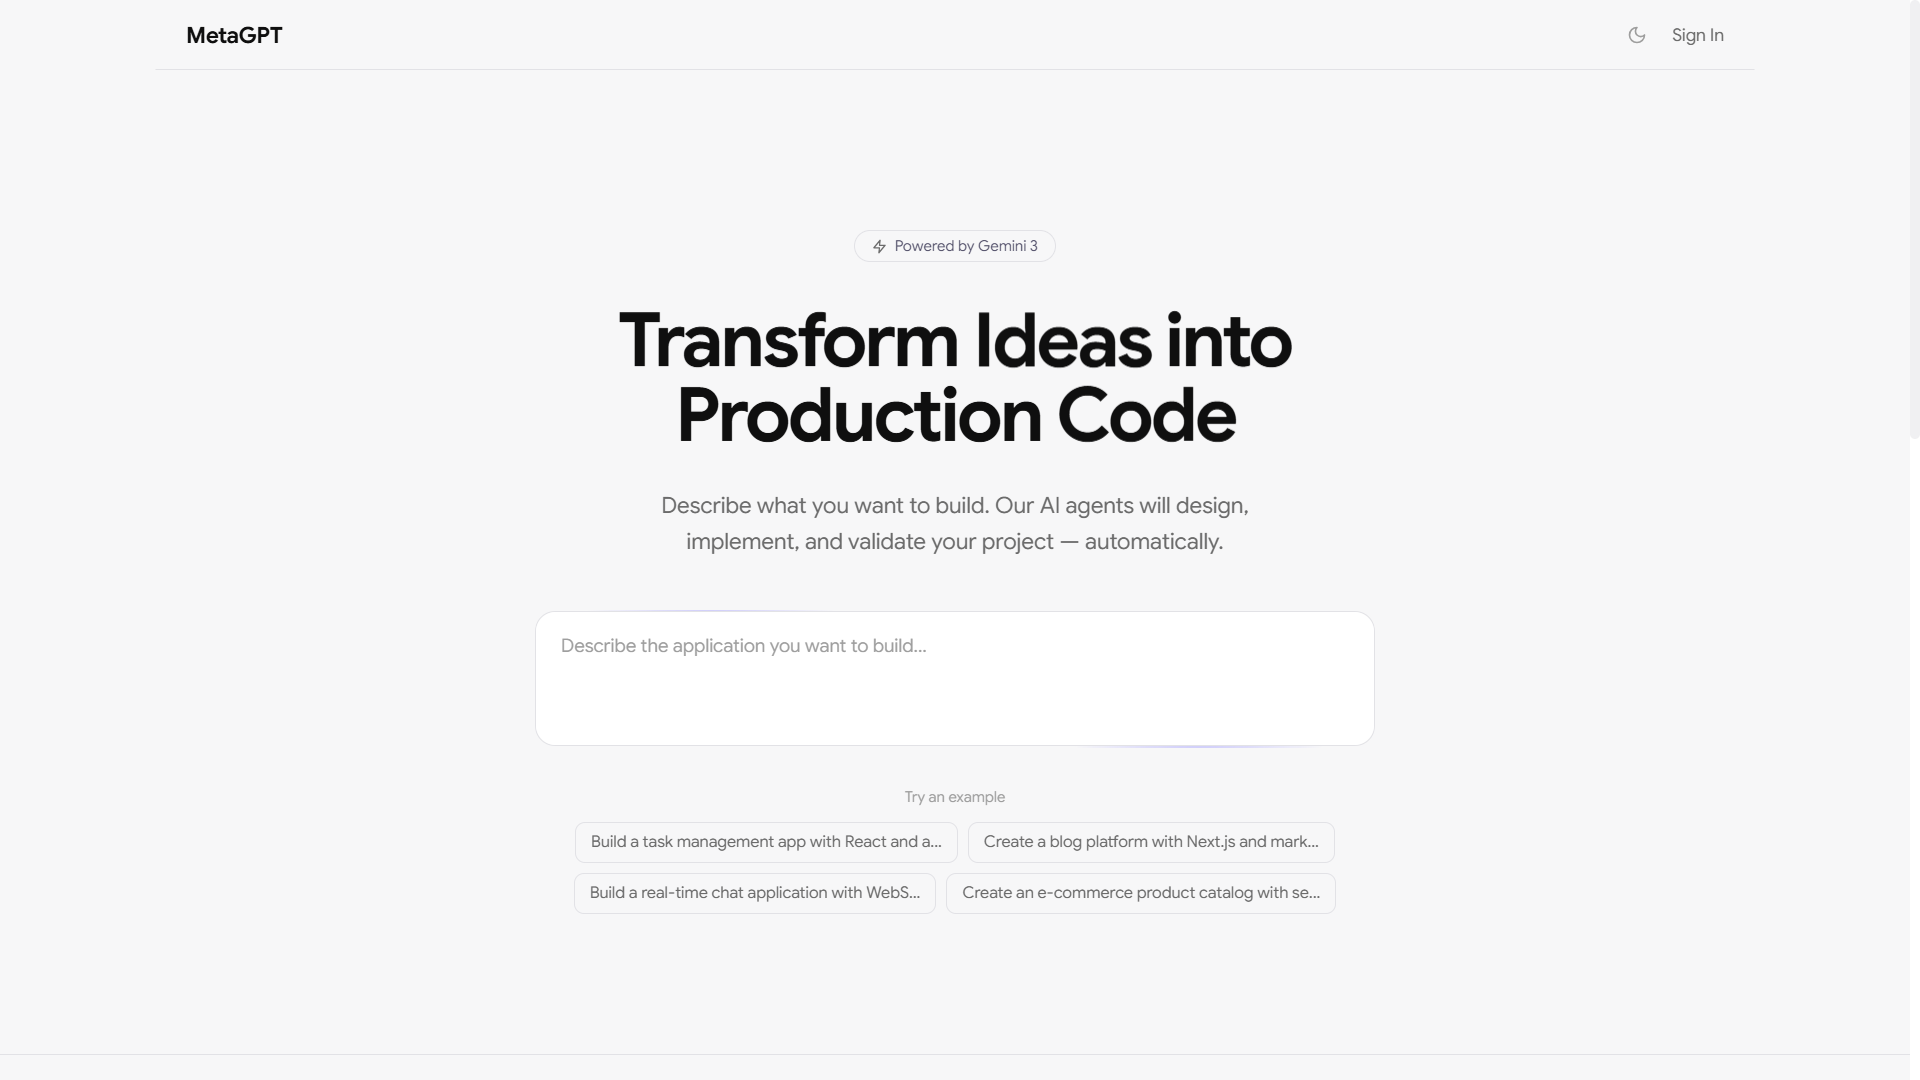
\includegraphics[width=1\textwidth]{images/home_page.png}
    \caption{MetaGPT — Home Page}
    \label{fig:ui_home}
\end{figure}

\vspace{1em}

\begin{figure}[H]
    \centering
    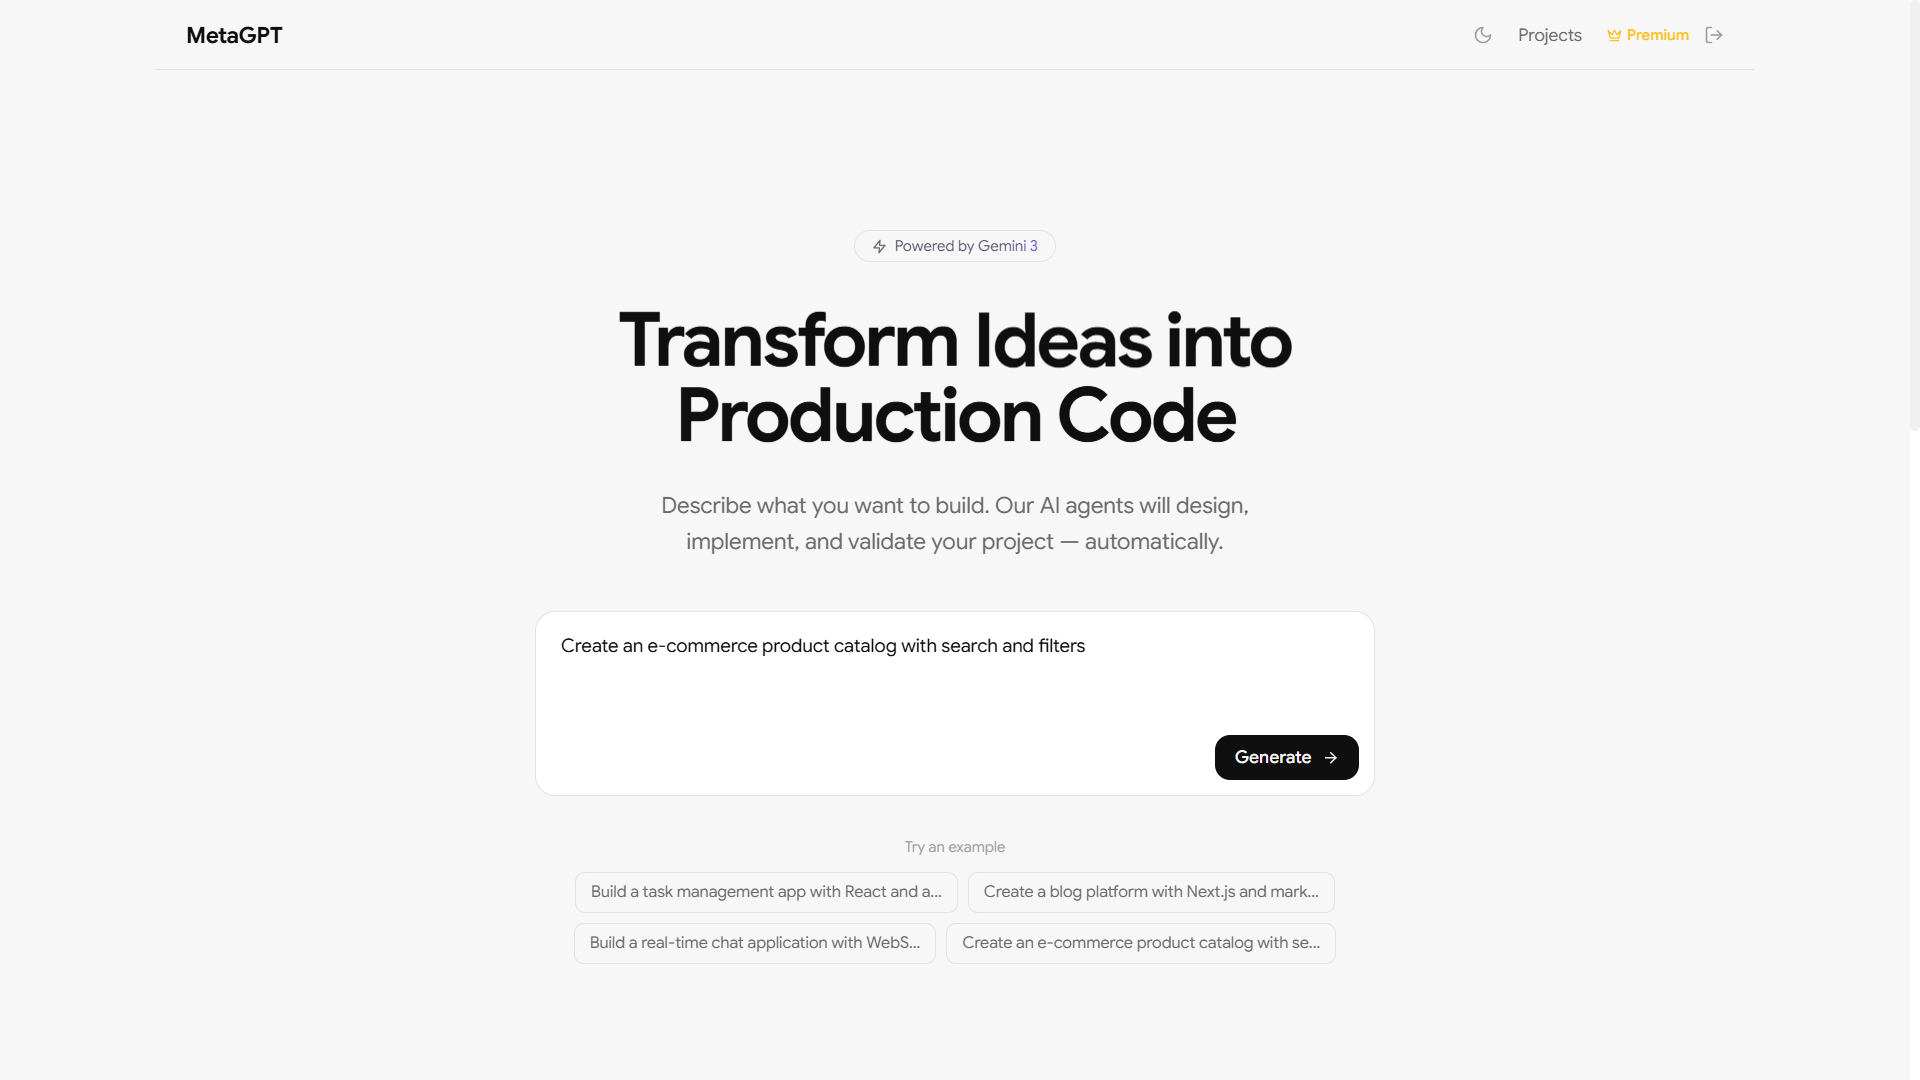
\includegraphics[width=1\textwidth]{images/home_page_with_prompt.png}
    \caption{MetaGPT — Home Page with Prompt Entered}
    \label{fig:ui_home_prompt}
\end{figure}

\vspace{1em}

\begin{figure}[H]
    \centering
    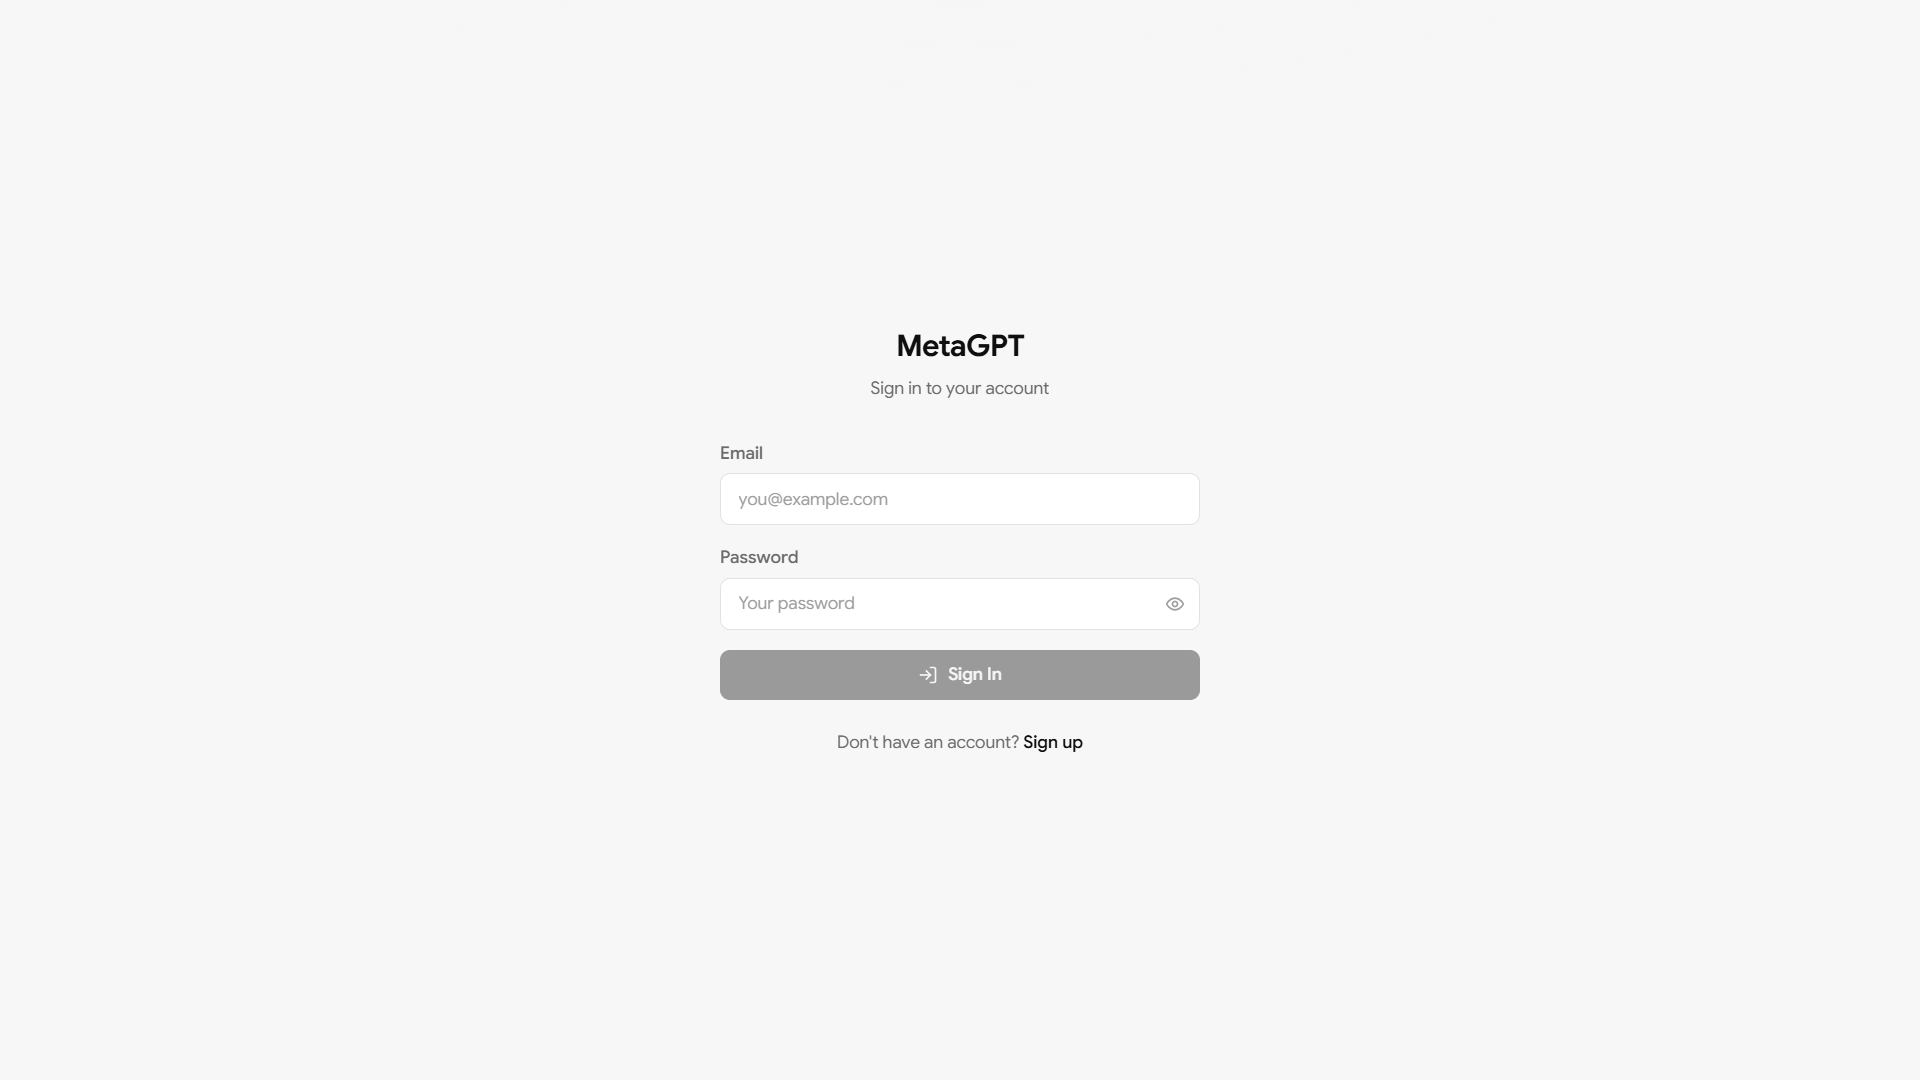
\includegraphics[width=1\textwidth]{images/signin_page.png}
    \caption{MetaGPT — Sign In Page}
    \label{fig:ui_signin}
\end{figure}

\vspace{1em}

\begin{figure}[H]
    \centering
    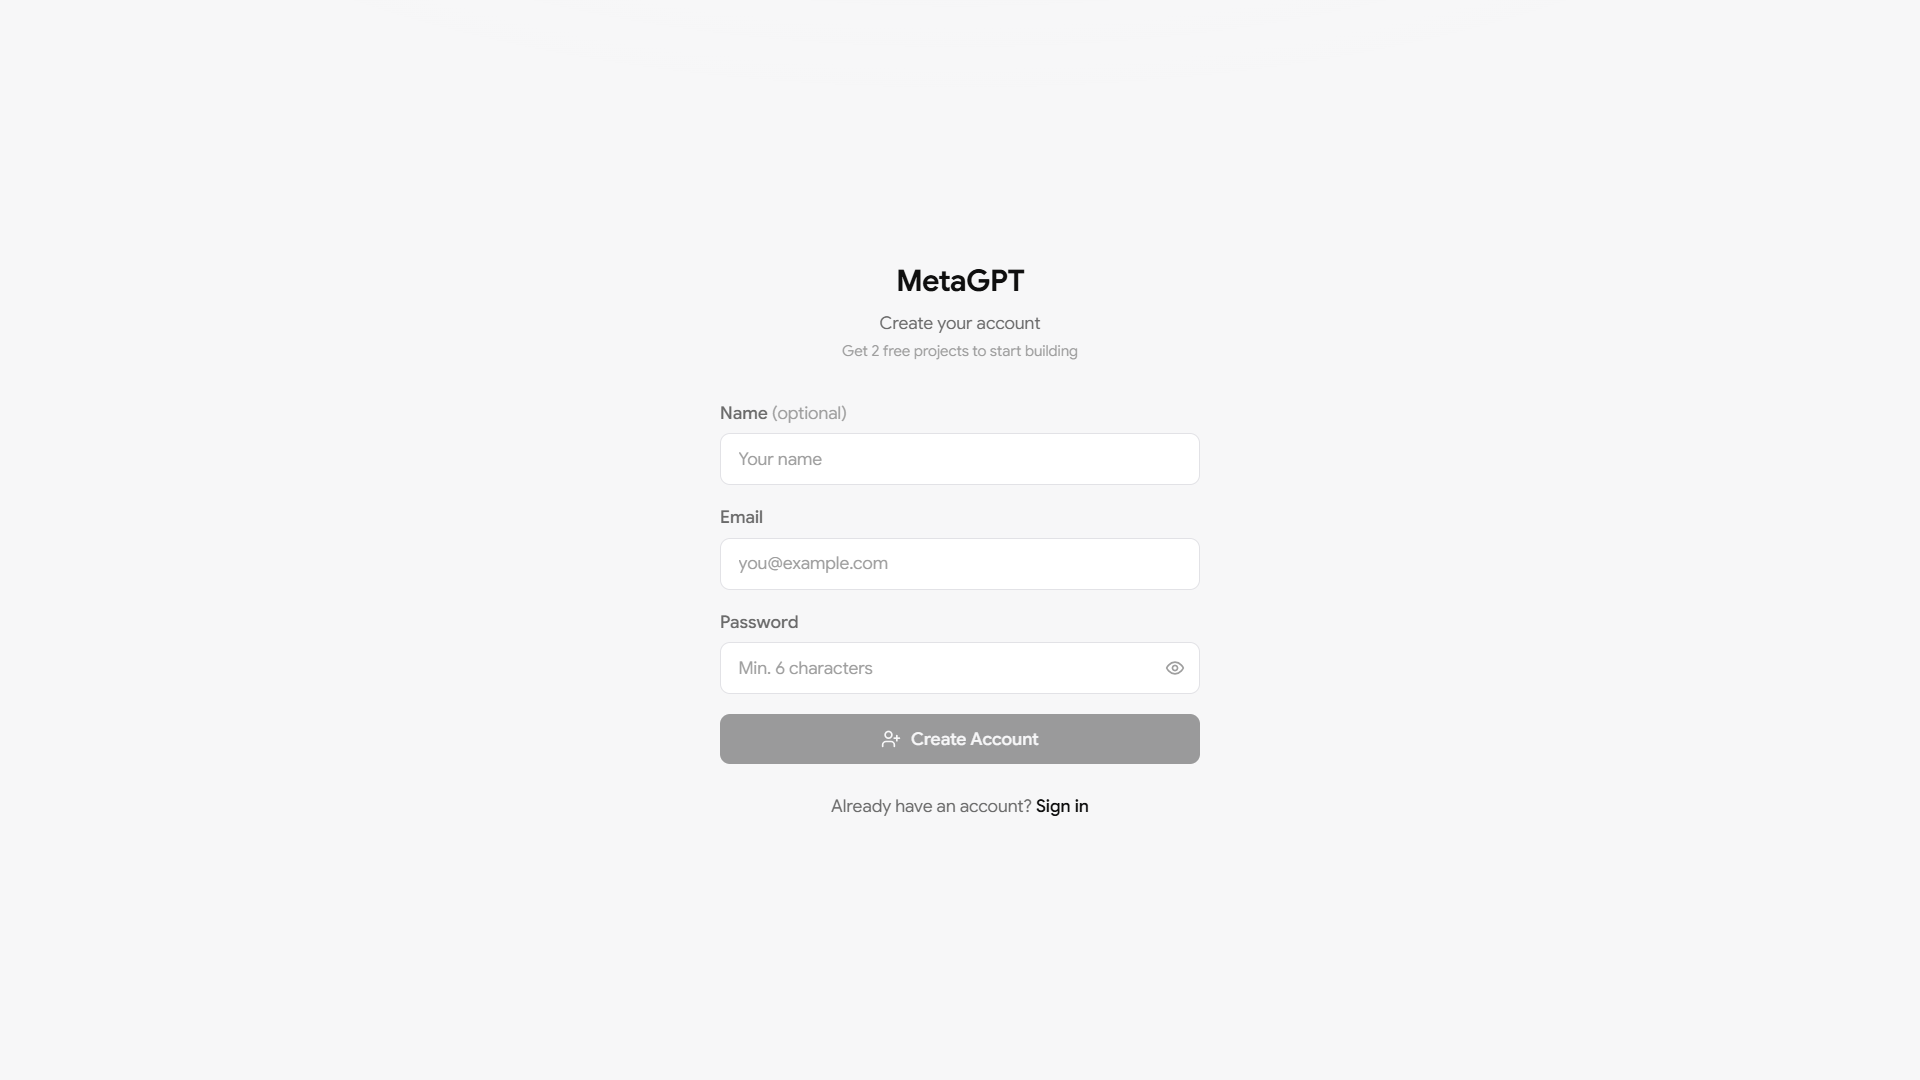
\includegraphics[width=1\textwidth]{images/signup_page.png}
    \caption{MetaGPT — Sign Up Page}
    \label{fig:ui_signup}
\end{figure}

\vspace{1em}

\begin{figure}[H]
    \centering
    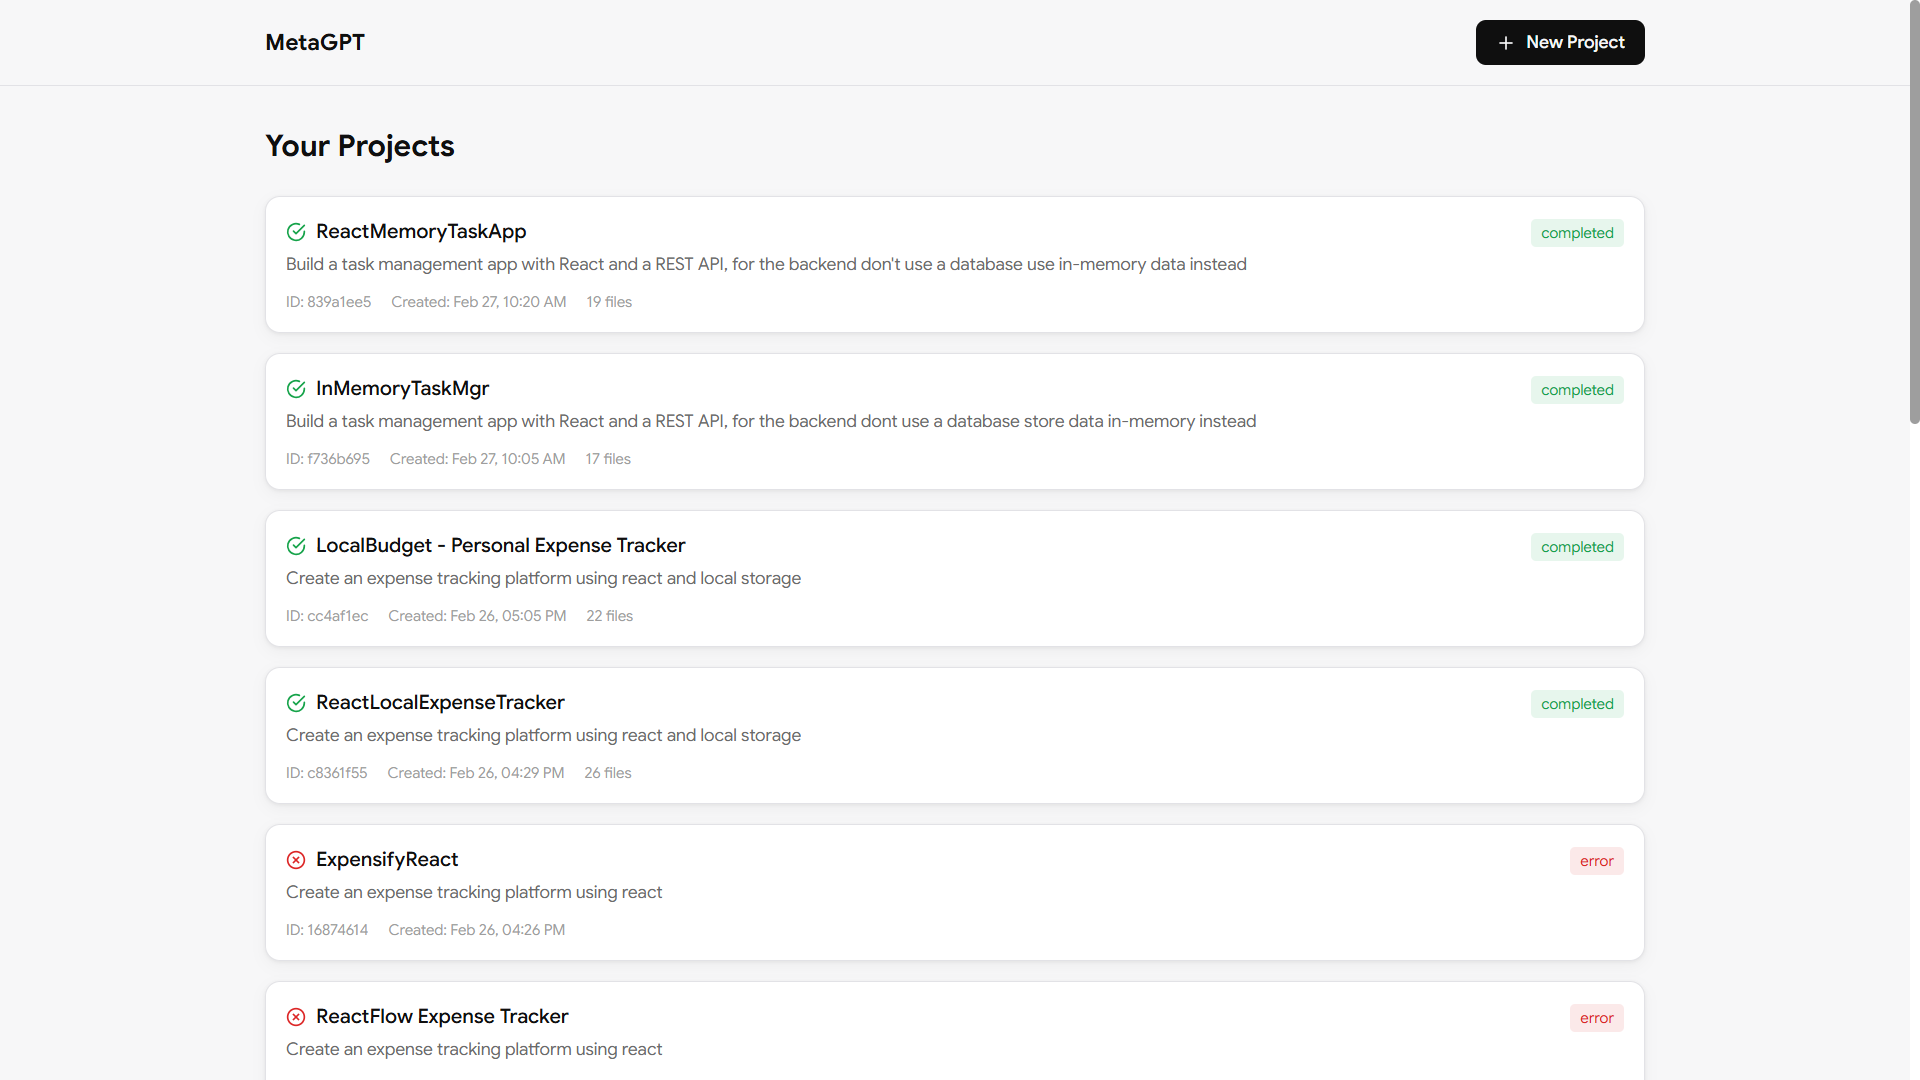
\includegraphics[width=1\textwidth]{images/list_of_projects.png}
    \caption{MetaGPT — List of Projects}
    \label{fig:ui_projects}
\end{figure}

\vspace{1em}

\begin{figure}[H]
    \vspace*{-\intextsep}
    \centering
    \captionsetup{aboveskip=0pt,belowskip=2pt}
    \caption{MetaGPT — Manager Agent Output}
    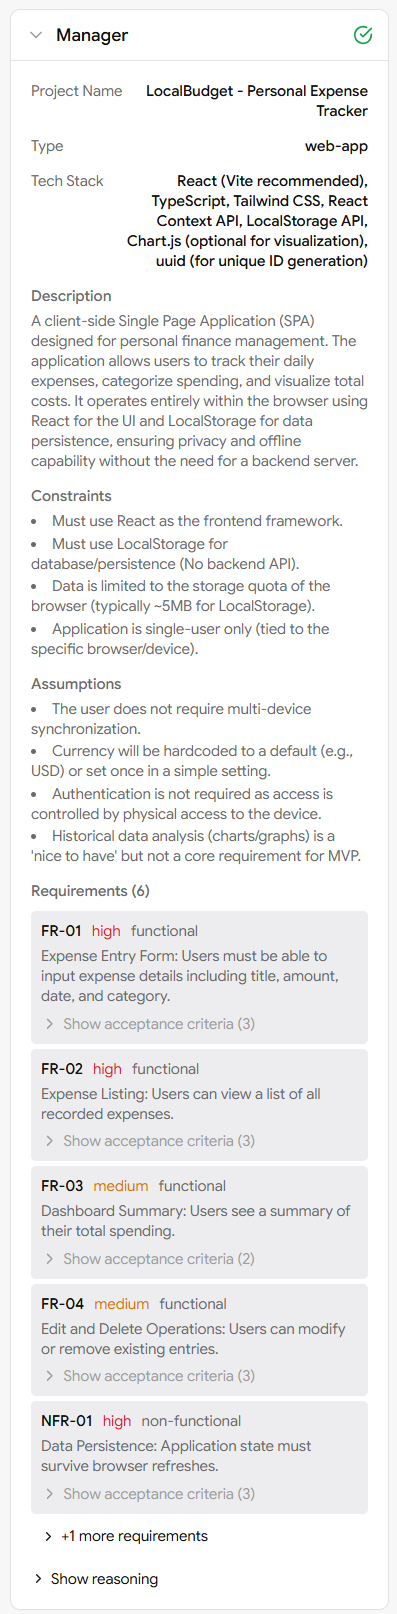
\includegraphics[height=\textheight,keepaspectratio]{images/manager_output.png}
    \label{fig:ui_manager}
\end{figure}

\vspace{1em}

\begin{figure}[H]
    \vspace*{-\intextsep}
    \centering
    \captionsetup{aboveskip=0pt,belowskip=2pt}
    \caption{MetaGPT — Architect Agent Output}
    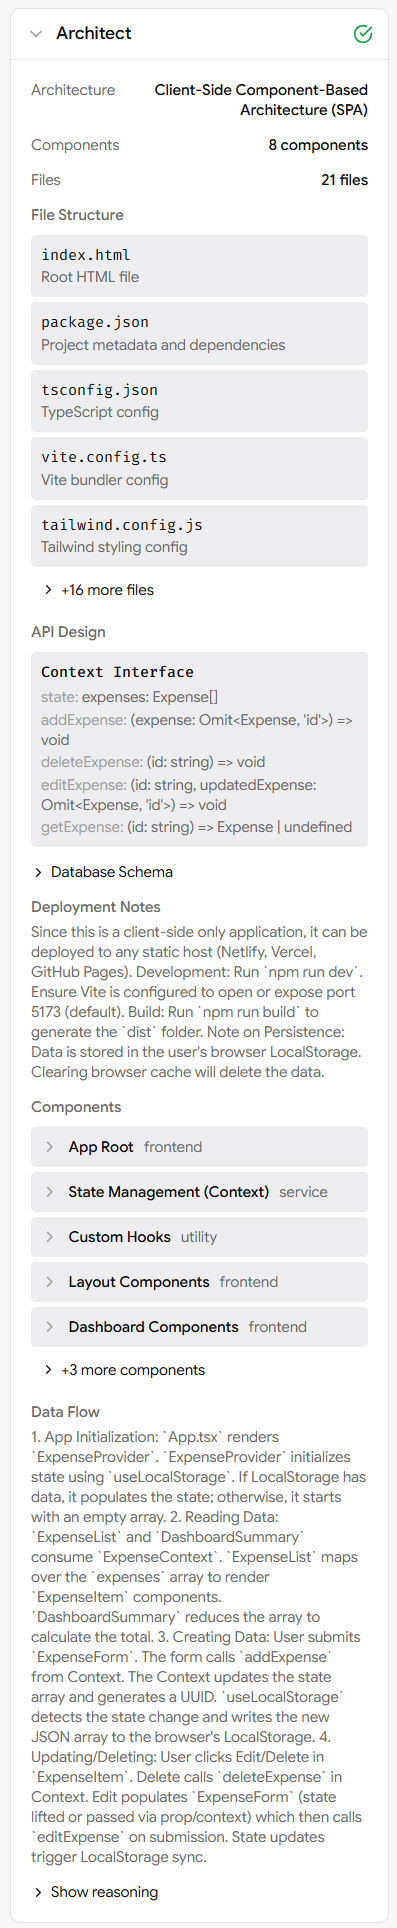
\includegraphics[height=\textheight,keepaspectratio]{images/architect_output.png}
    \label{fig:ui_architect}
\end{figure}

\vspace{1em}

\begin{figure}[H]
    \vspace*{-\intextsep}
    \centering
    \captionsetup{aboveskip=0pt,belowskip=2pt}
    \caption{MetaGPT — Engineer Agent Output}
    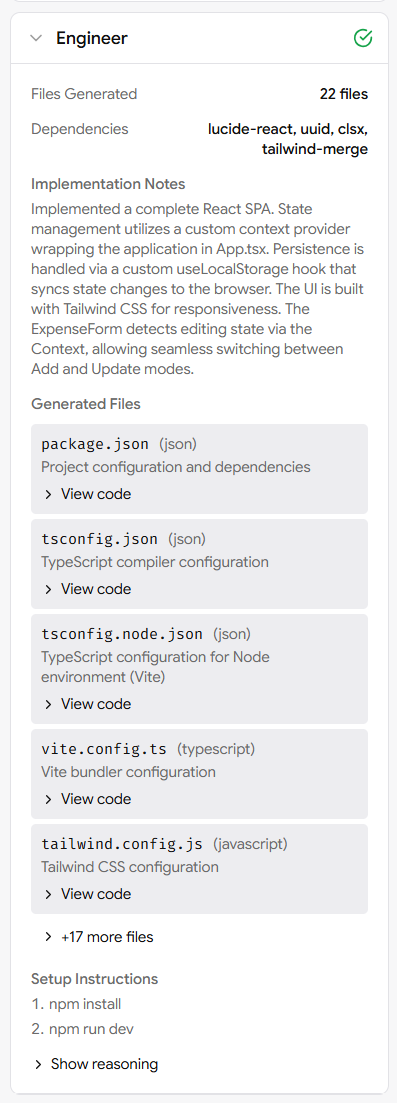
\includegraphics[height=\textheight,keepaspectratio]{images/engineer_output.png}
    \label{fig:ui_engineer}
\end{figure}

\vspace{1em}

\begin{figure}[H]
    \vspace*{-\intextsep}
    \centering
    \captionsetup{aboveskip=0pt,belowskip=2pt}
    \caption{MetaGPT — QA Agent Output}
    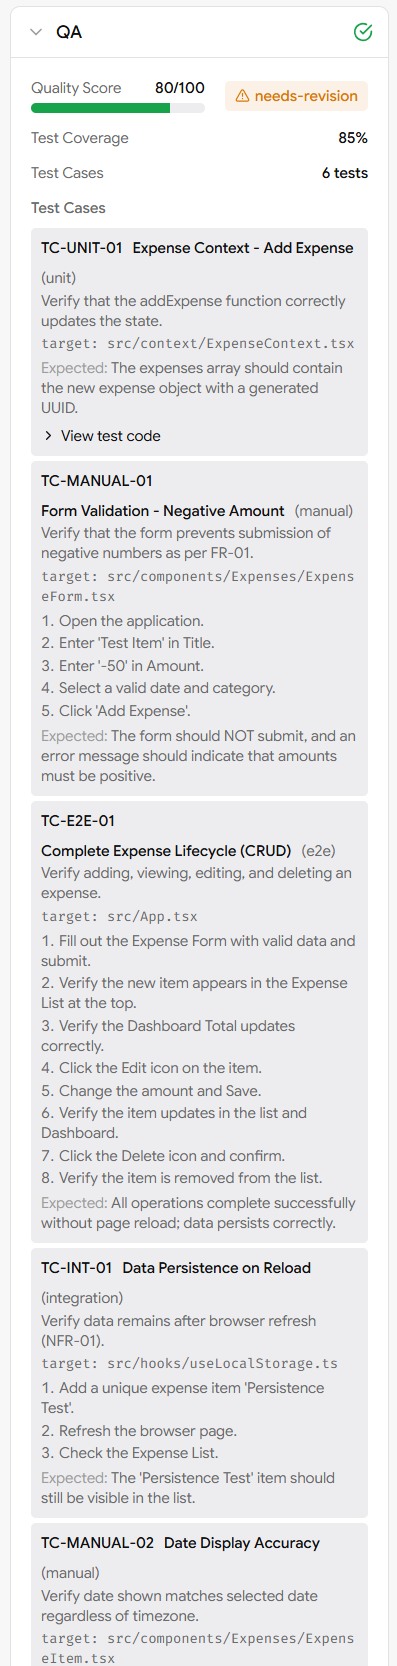
\includegraphics[height=\textheight,keepaspectratio]{images/qa_output_1.png}
    \label{fig:ui_qa}
\end{figure}

\begin{figure}[H]
    \vspace*{-\intextsep}
    \centering
    \captionsetup{aboveskip=0pt,belowskip=2pt}
    \caption{MetaGPT — QA Agent Output (continued)}
    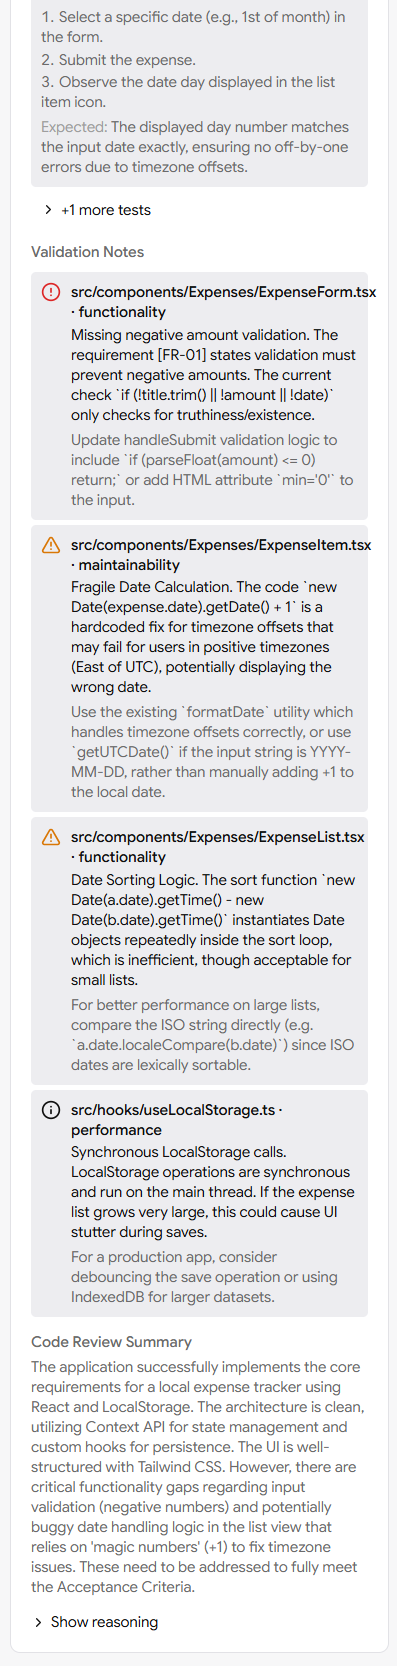
\includegraphics[height=\textheight,keepaspectratio]{images/qa_output_2.png}
    \label{fig:ui_qa_2}
\end{figure}

\vspace{1em}

\begin{figure}[H]
    \centering
    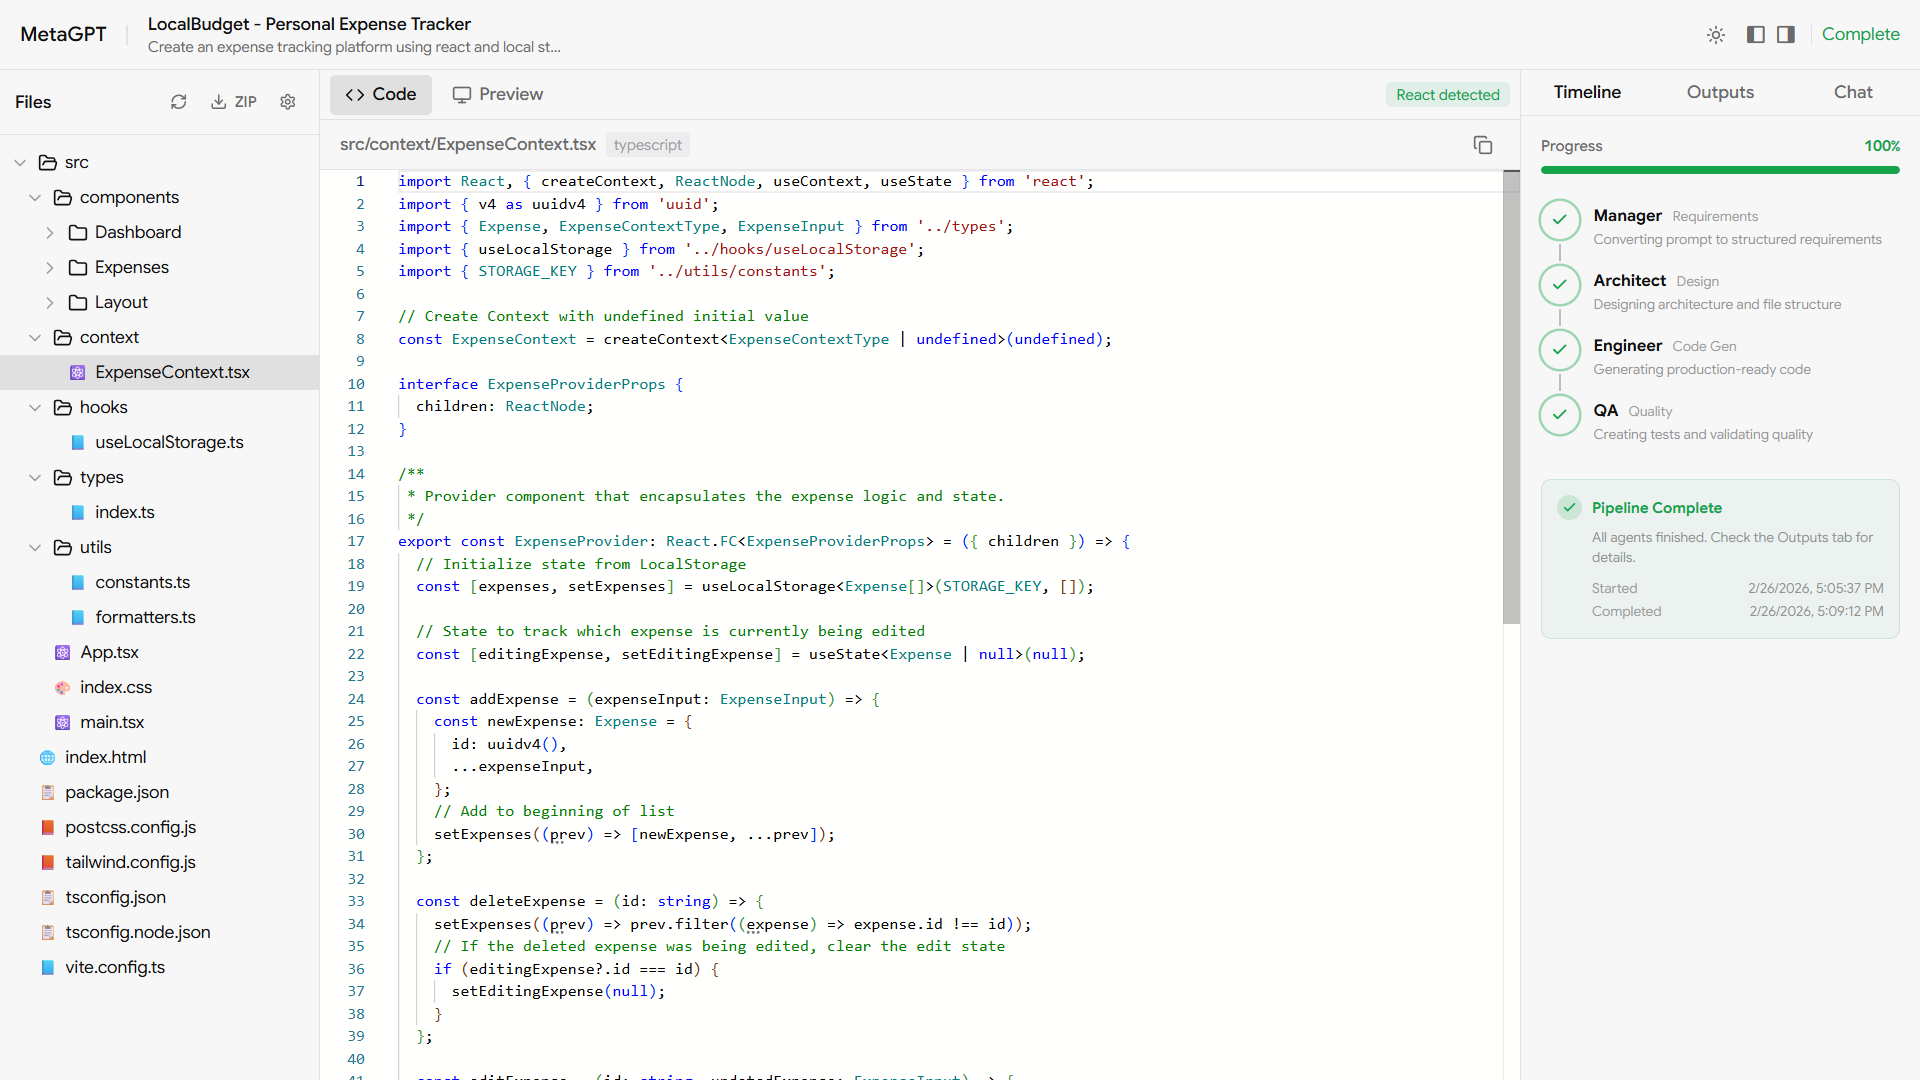
\includegraphics[width=1\textwidth]{images/code_preview.png}
    \caption{MetaGPT — Code Preview}
    \label{fig:ui_code}
\end{figure}

\vspace{1em}

\begin{figure}[H]
    \centering
    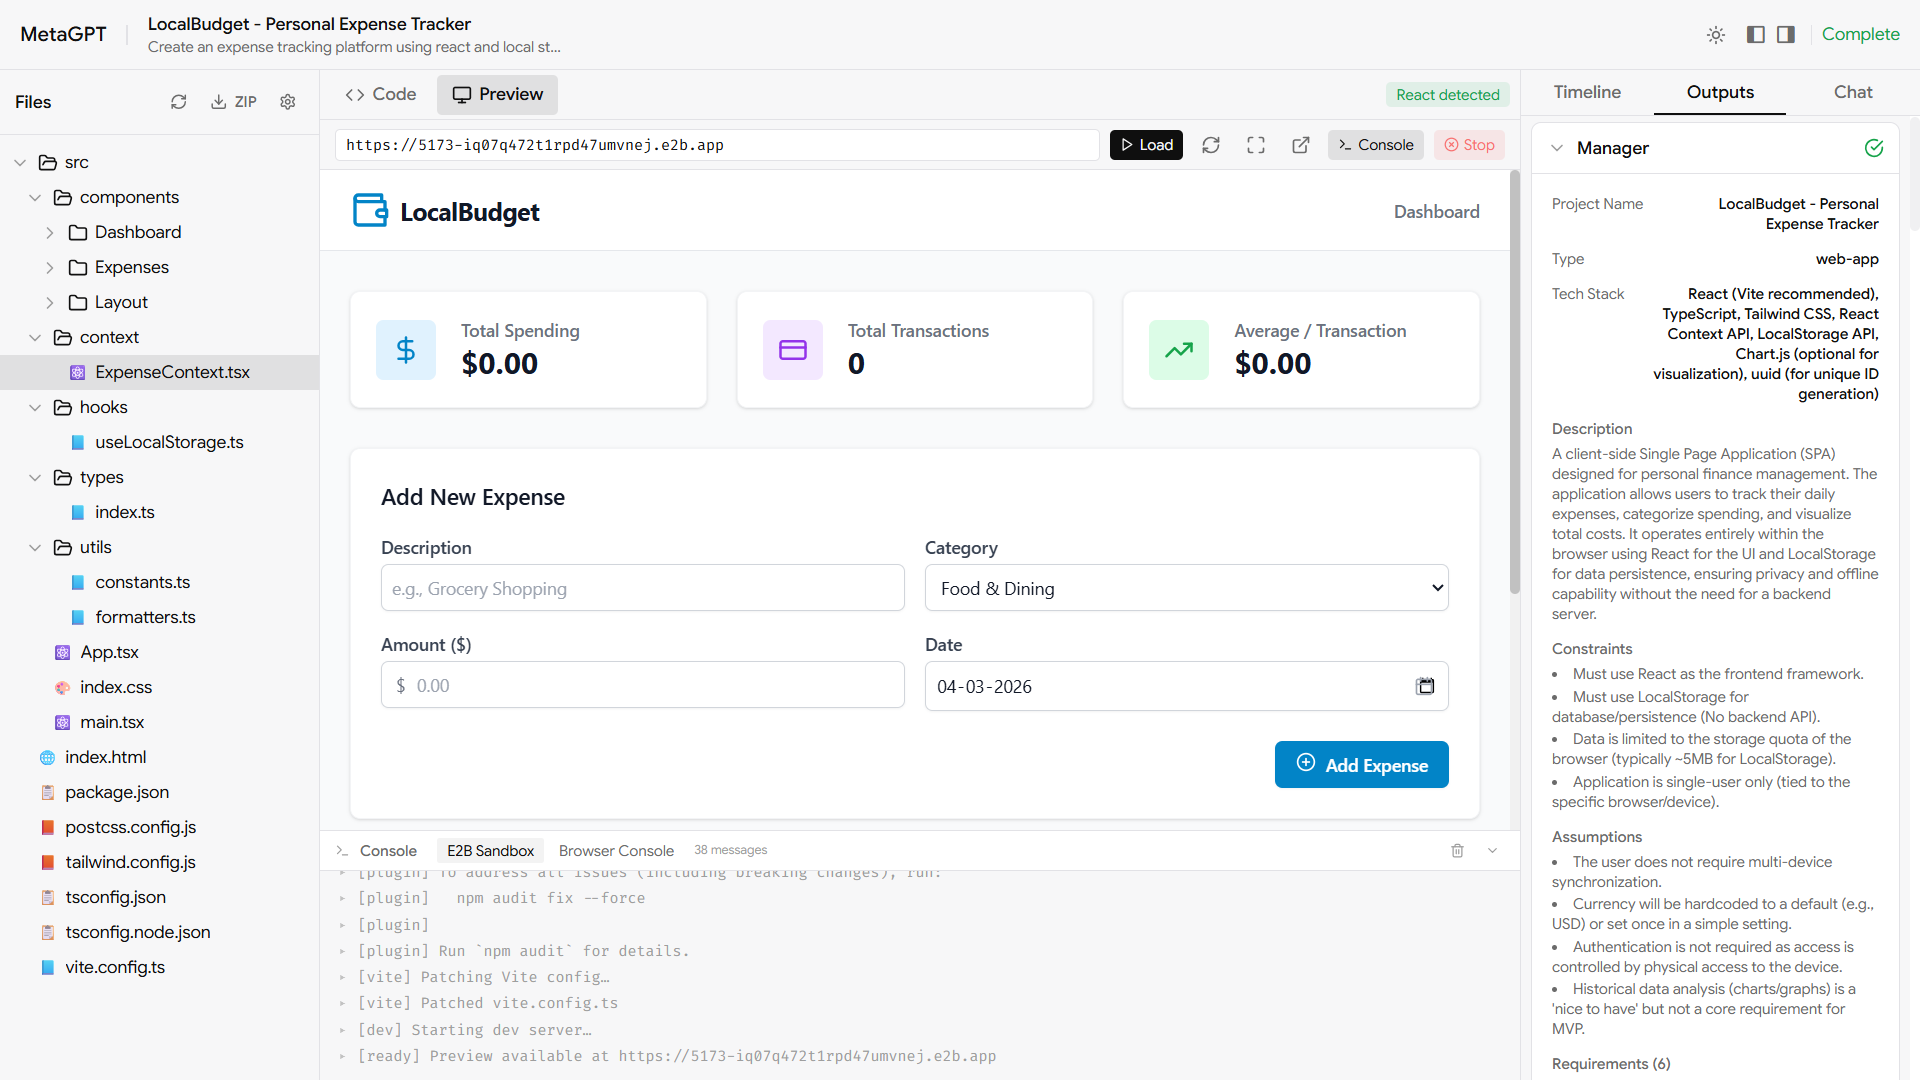
\includegraphics[width=1\textwidth]{images/sandbox_live_preview.png}
    \caption{MetaGPT — Sandbox Live Preview}
    \label{fig:ui_sandbox}
\end{figure}

